\documentclass[../main.tex]{subfiles}


\begin{document}

\section{Evaluation}

\subsection{Test Result Without Machine Learning}

In the process of finding test data, there is a benchmark of Detection of Software Clones: {\color{blue} \url{http://www.bauhaus-stuttgart.de/clones/}}. It is a general repository and information center for Detection of Software Clones, it accepts files with labeled clones for clone detection tool evaluation. However its format does not meet our requirement, so again we use manual selection to find ``ground truth'' for testing, just as we did in finding training data: using a low threshold of 0.65 to rule out most of the pairs and manually compare the rest.

Using low threshold to rule out most of the non-clones is reasonable because STCD can also work without training. Apply STCD to test files without training will get the following result:


Test Files: Spinner.java \\
Similarity = 0.98 \\

Line \#: 304-313 \\
public void cut () { \\
	if ((style \& SWT.READ\_ONLY) != 0) return; \\ \indent
	NSText fieldEditor = textView.currentEditor(); \\
	if (fieldEditor != null) { \\ \indent
		fieldEditor.cut(null); \\
	\} else \{ \\ \indent
		//TODO \\
	\} \\
} \\

Line \#: 563-572
public void paste () {
	checkWidget ();
	if ((style \& SWT.READ\_ONLY) != 0) return;
	NSText fieldEditor = textView.currentEditor();
	if (fieldEditor != null) {
		fieldEditor.paste(null);
	} else {
		//TODO
	}
}

Test Files: Tree.java
Similarity = 0.89

Line \#: 368-377
void clear (TreeItem parentItem, int index, boolean all) {
	TreeItem item = \_getItem (parentItem, index, false);
	if (item != null) {
		item.clear();
		item.redraw (-1);
		if (all) {
			clearAll (item, true);
		}
	}
}

Line \#: 379-391
void clearAll (TreeItem parentItem, boolean all) {
	int count = getItemCount (parentItem);
	if (count == 0) return;
	TreeItem [] children = parentItem == null ? items : parentItem.items; 
	for (int i=0; i<count; i++) {
		TreeItem item = children [i];
		if (item != null) {
			item.clear ();
			item.redraw (-1);
			if (all) clearAll (item, true);
		}
	}
}

These two pairs are clones and are found by our tool. After manual inspection, we found that almost all pairs with similarity lower than 0.65 are not clones. Actually, many pairs with similarity between 0.65 and 0.87 are not clones either. So we consider the process of manually finding ground truth is realiable, and the clones ruled out by the similarity of 0.65, i.e. false negative, is small.

\subsection{Test Result With Machine Learning}

We select test data from SWT--since machine learning is based on SWT files. The 10 files we used for testing are: \textit{Button.java, CoolBar.java, Menu.java, Spinner.java, TabFolder.java, TableItem.java, ToolBar.java, ToolItem.java, Tracker.java, Tree.java}. The number of methods ranges from 38 to 147.

Since we have our tool and test data, we are ready to do evaluation. After tranining with MLP, the test result is shown in Table \ref{tab:Table_2}: \\

\begin{tablehere}
%\small
\begin{tabular}[h]{|c|c|c|c|}
\hline
Test Files & \begin{tabular}{c}TP + FN \\ (Actual \\ Clones) \end{tabular} 
				& \begin{tabular}{c}TP + FP \\ (Detected \\ Clones) \end{tabular} & TP \\
\hline
Button.java & 0 & 4 & 0 \\
\hline
CoolBar.java & 11 & 12 & 10\\
\hline
Menu.java &1 & 0 & 0\\
\hline
Spinner.java & 2 & 2 & 2\\
\hline
TabFolder.java & 3 & 2 & 2 \\
\hline
TableItem.java & 20 & 20 & 18\\
\hline
ToolBar.java & 4 & 4 & 4 \\
\hline
ToolItem.java & 3 & 3 & 3 \\
\hline
Tracker.java & 1 & 1 & 1 \\
\hline
Tree.java & 11 & 13 & 9\\
\hline
\end{tabular}\\
\caption{Test Result}\label{tab:Table_2}
\end{tablehere}

Here we used a threshold of 0.87. A lower threshold will result in more ``clones'' to be detected, which reduces the precision rate, while a higher threshold will result in more false negatives, thus a lower recall rate. After actual testing, a threshold of 0.87 balances the precision and recall rate.

In the table above, the detected clones are very close to actual clones, 4 out of 10 files got exact match.

One thing needs to be mentioned is about \textit{ToolItem.java}, the process of manually finding ``ground truth'' results in 2 false negatives. At first we decided there is only 1 ``actual'' clone, but after training and testing, STCD found 3. After checking by eye, we decided the extra 2 pairs are actually clones, they were ruled out earlier by the low threshold of 0.65. This being said, manual selection does result in false negatives, however on the other hand, this implies the training process is effective.

\subsection{Precision and Recall}

\begin{figurehere}
\centering 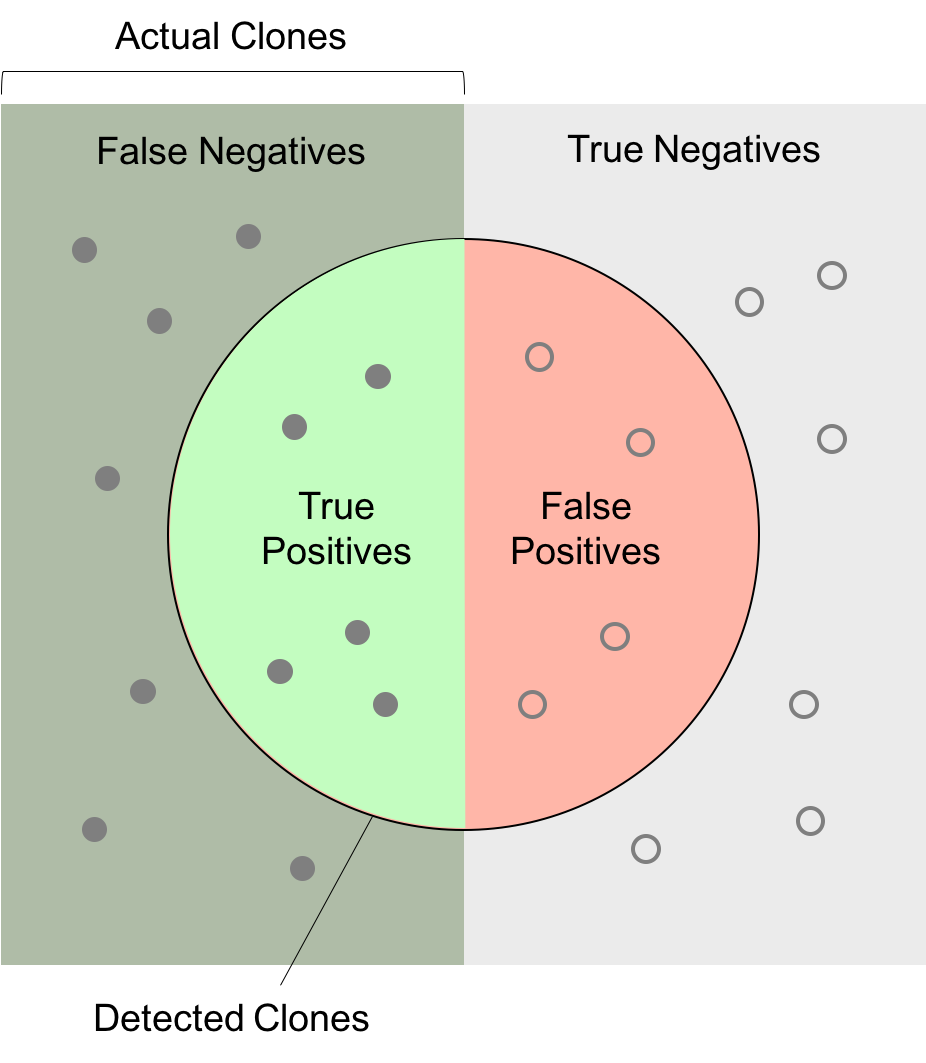
\includegraphics[width = 0.4 \textwidth]{Graph_4} 
\caption{Calculation of Precision and Recall} \label{fig:Graph_4}
\end{figurehere}

Fig:\ref{fig:Graph_4} shows the relationship between actual clones and detected clones, based on the definition of Precision and Recall, 

\begin{equation}
\text{Precision} = \frac{ \text{True Positives}} {\text{Detected Clones}} = \frac{ \text{TP}} {\text{TP} + \text{FP}}
\end{equation}

\begin{equation}
\text{Recall} = \frac{ \text{True Positives}} {\text{Actual Clones}} = \frac{ \text{TP}} {\text{TP} + \text{FN}}
\end{equation}

Except for \textit{Button.java} and \textit{Menu.java} which we are unable to calculate the Precision and Recall, the other 8 files have Average Precision of 92.75\% and Average Recall of 91.25\%. The precision and recall for each file is given in Fig:\ref{fig:Graph_5}, they are high enough to make STCD practical.

\begin{figurehere}
\centering 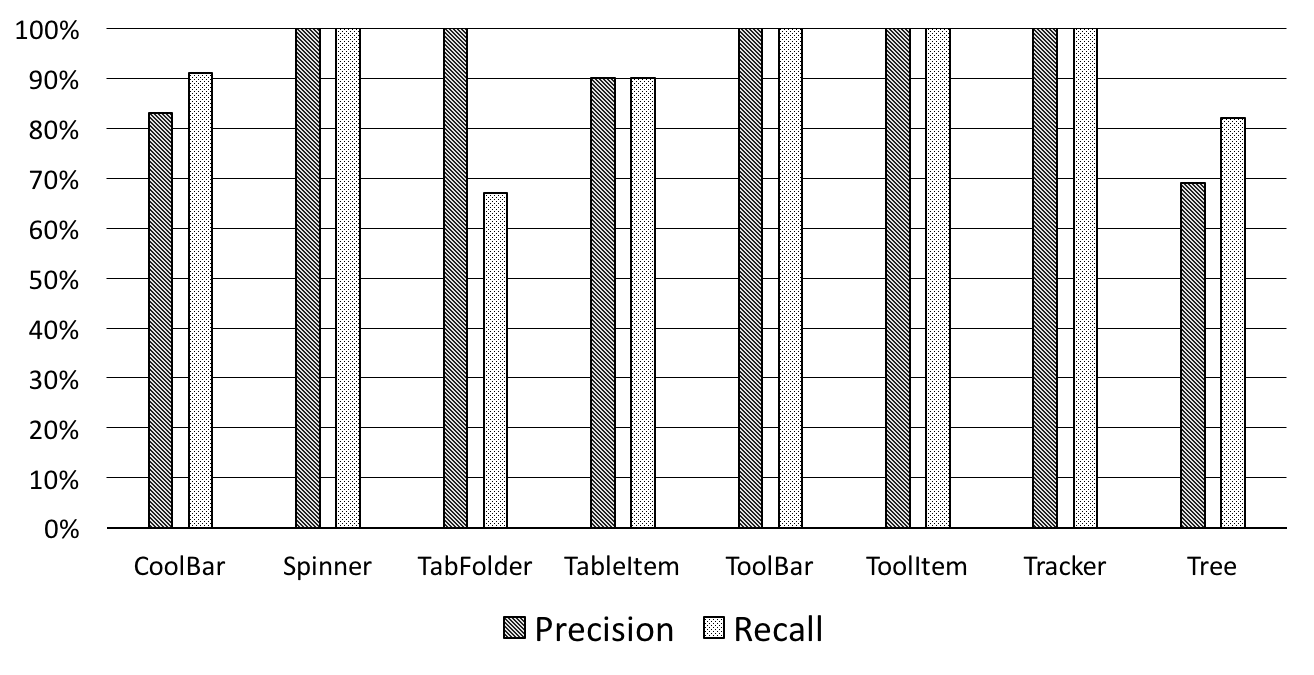
\includegraphics[width = 0.45 \textwidth]{Graph_5} 
\caption{Precision and Recall of STCD} \label{fig:Graph_5}
\end{figurehere}

\subsection{Time Cost Evaluation}

The time cost of STCD is also evaluated, and is given in Fig:\ref{fig:Graph_6}. This experiment is performed on a Macbook Air, time cost varies with the configuration of computer. Since the comparasion for n methods is $\frac{n(n-1)}{2}$, we expect the time cost to be quadratic, and it turns out to be so--with some variations, which is the result of different method lengths.

A quadratic time cost is tolerable, especially with the fact that running a file with 100 methods takes only 2 seconds. Most Java files won't have more than hundreds of methods, so our tool is very practical.

\begin{figurehere}
\centering 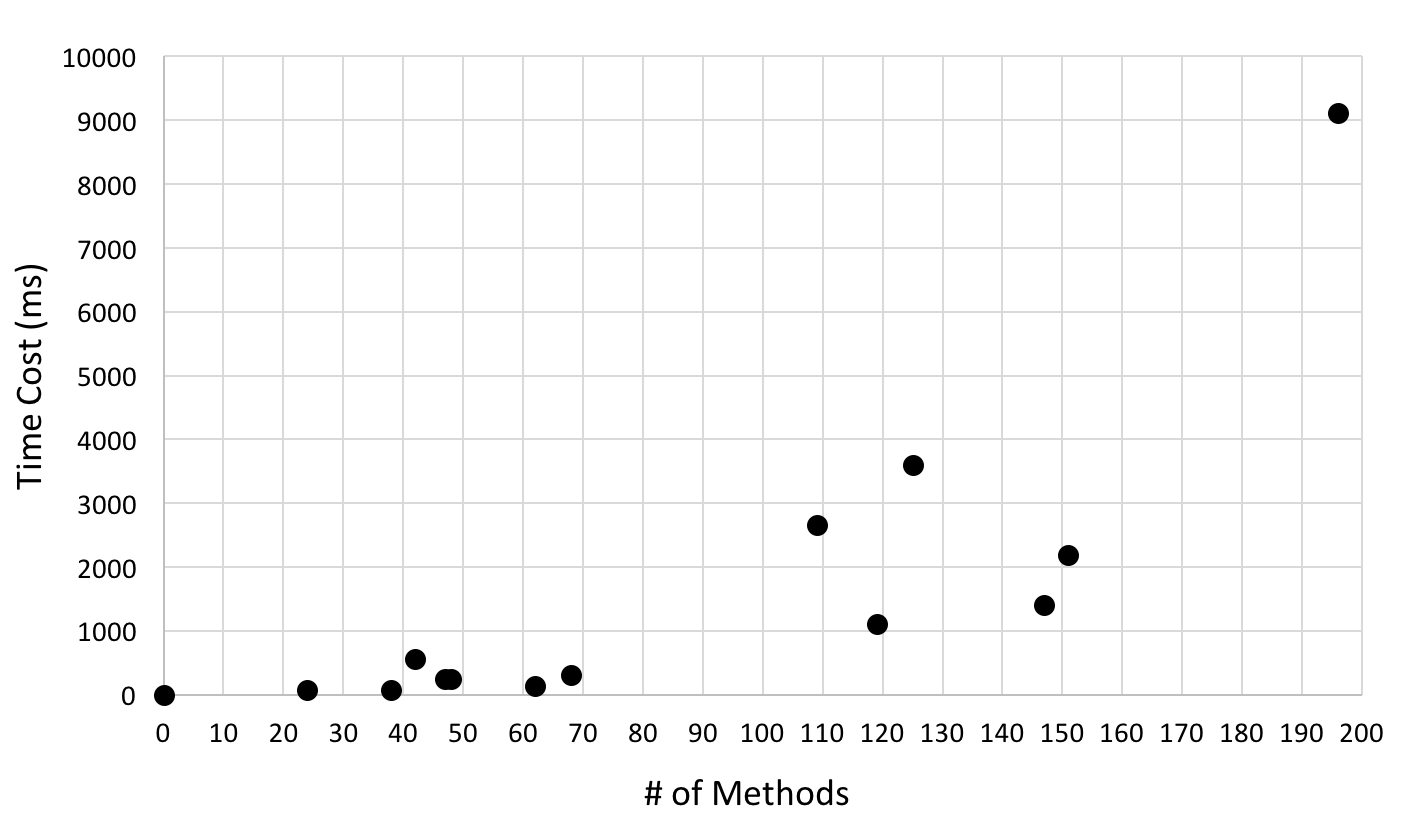
\includegraphics[width = 0.45 \textwidth]{Graph_6} 
\caption{Time Cost of STCD} \label{fig:Graph_6}
\end{figurehere}

\end{document}